\documentclass{article}

\usepackage{graphicx}
\graphicspath{ {images/} }

\title{Ground-Truth Injection for Peer Grading using the Vancouver Algorithm}
\author{Donald "Drew" Bronson}
\date{2016-05-06}

\begin{document}
	\maketitle
	\pagenumbering{arabic}
	

	\section{Simulation Parameters}
	The simulations below were run with the following default parameters:
	\begin{itemize}
		\item There are twenty group submissions.
		\item There are three students per group.
		\item Each student grades three assignments.
		\item The simulation is run two hundred times and the data aggregated.
		\item The legend indicates the number of ground-truth grades supplied to the algorithm.
		\item The default method for choosing ground truth grades is to select them uniformly at random.
		\item Methods for choosing ground truth grades are applied after the entire cover has been chosen. If the cover is smaller than the number of ground truth grades allowed, the grades used are chosen uniformly at random from those in the cover.
		\item Peer quality is represented by the number of draws a peer gets from a uniform distribution on the range (0, 1).
		\item Peer quality is uniformly random on the range [1, 5].
		\item The true value of a submission's grade is always 0.5, the expectation of a uniform distribution on the range (0, 1).
		\item The grading algorithm used is the Vancouver algorithm, and it is terminated after ten iterations.
		\item The statistic plotted is the CDF of submission grade error, the quantity abs(submission grade from algorithm - 0.5).
		\item The default number of ground truths is the tuple (0, 5, 10, 15) and should plot four CDFs per plot.
		\item Each plot runs its own batch of simulations.
	\end{itemize}
	

	\section{Initial Verification of Vancouver Algorithm}
	The first thing to be done was to verify the number of iterations needed for Vancouver to converge to a reasonable output. Ten was hypothesized to be an appropriate number of iterations based on earlier simulations conducted by other members of the research group, and the simulations I conducted support this hypothesis. Figure \ref{fig:vancouver-10-steps} is the graph for ten iterations and Figure \ref{fig:vancouver-20-steps} is the graph for twenty iterations. As you can see, there is no significant difference between them. I have also included the graph for a single iteration, which represents simple averaging, in Figure \ref{fig:vancouver-1-step}. This shows that for the default simulation parameters, simple averaging has comparable performance to Vancouver. All of the plots below were run with the number of Vancouver iterations specified and the remaining settings default as described above.

	\begin{figure}[h]
		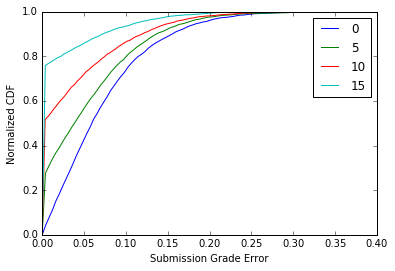
\includegraphics{vancouver-10-steps.png}
		\caption{Ten-Iteration Vancouver}
		\label{fig:vancouver-10-steps}
	\end{figure}
	
	\begin{figure}[h]
		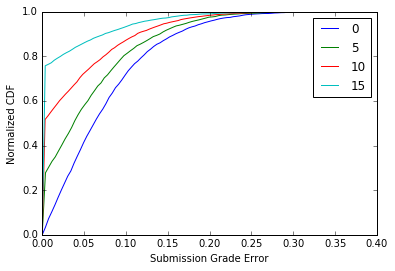
\includegraphics{vancouver-20-steps.png}
		\caption{Twenty-Iteration Vancouver}
		\label{fig:vancouver-20-steps}
	\end{figure}
	
	\begin{figure}[h]
		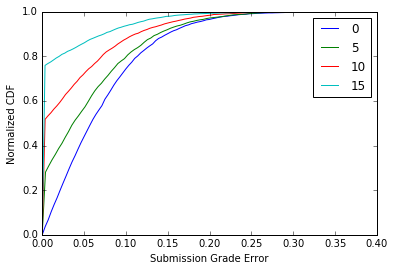
\includegraphics{vancouver-1-step.png}
		\caption{One-Iteration Vancouver (Simple Averaging)}
		\label{fig:vancouver-1-step}
	\end{figure}
	

	\section{Evaluation of Vancouver with Injected Ground Truths}
	As may be evident from the plots already shown, Vancouver does not appear to perform better with more ground truths; the entirety of the observable increase in performance can be attributed to the direct linear decrease in mean error that results from inserting more true grades. The graph shown is a plot of the expected mean error calculated from 100 trials with the other parameters default. See Figure \ref{fig:vancouver-vs-ground-truth-cover}.
	
	\begin{figure}[h]
		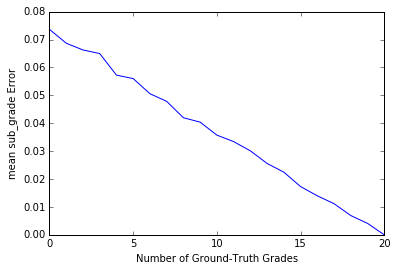
\includegraphics{vancouver-vs-ground-truth-cover.png}
		\caption{Vancouver as Number of Ground Truth Grades Increases}
		\label{fig:vancouver-vs-ground-truth-cover}
	\end{figure}
	

	\section{Evaluation of Vancouver with Grading a Cover}
	The simulations up until this point have assumed that a cover should be graded first before subsequent ground truths are chosen randomly, but this was not the initial case. Rather, in my first run of simulations, I chose assignments to inject ground truth for in a uniformly random manner, ignoring the existence of a cover. A plot of this is shown in Figure \ref{fig:vancouver-vs-ground-truth-no-cover}, and does not appear noticeably different from Figure \ref{fig:vancouver-vs-ground-truth-cover}, indicating that there may be little to no benefit of grading a cover first, other than that it allows for grading of the graders. I also include plots of both of their CDFs for comparison to each other in Figures \ref{fig:vancouver-no-cover} and \ref{fig:vancouver-cover-random}. Again, there is no discernible difference between the two figures.
	
	\begin{figure}[h]
		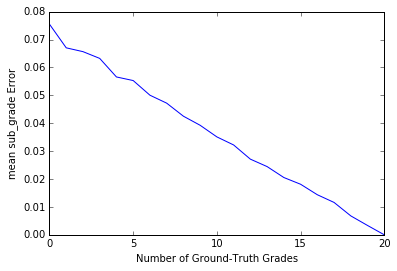
\includegraphics{vancouver-vs-ground-truth-no-cover.png}
		\caption{Vancouver as Number of Ground Truth Grades Increases (No Cover)}
		\label{fig:vancouver-vs-ground-truth-no-cover}
	\end{figure}
	
	\begin{figure}[h]
		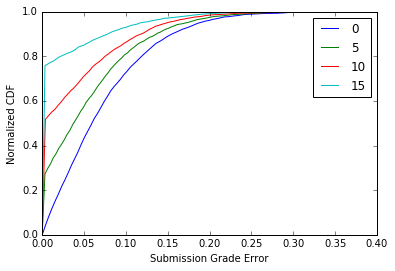
\includegraphics{vancouver-no-cover.png}end{document}
		\caption{Vancouver (No Cover)}
		\label{fig:vancouver-no-cover}
	\end{figure}
	
	\begin{figure}[h]
		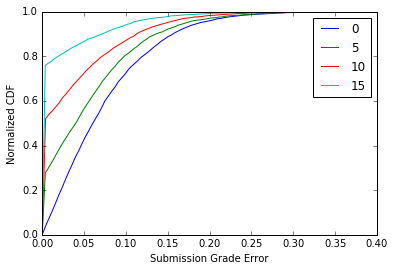
\includegraphics{vancouver-cover-random.png}
		\caption{Vancouver (With Cover and Random Selection Past Cover)}
		\label{fig:vancouver-cover-random}
	\end{figure}
	
	
	\section{Attempts to Find a Distribution for Which Ground Truth Injection is Better than Default}
	I next attempted to find a distribution for which ground truth injection would be more helpful than it is for the default uniform distribution on the range [1, 5]. Distributions that I tried included bimodal (Figure \ref{fig:vancouver-bimodal}) and skewed both low and high (Figures \ref{fig:vancouver-skewed} and \ref{fig:vancouver-skewed-low}). None of these distributions showed noticeable improvements over the default. It is worth noting for the sake of clarity that minor differences in the overall error are visible here, but this is due to the initial input from the graders being better or worse, since I was changing the distribution of quality of the graders.
	
	\begin{figure}[h]
		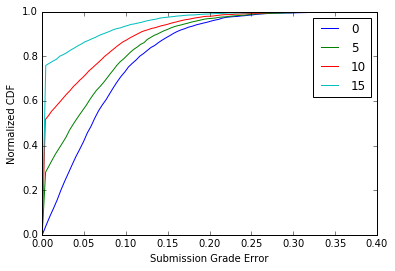
\includegraphics{vancouver-bimodal.png}
		\caption{Vancouver (With Peer Quality Drawn Uniformly from the Set \{1, 5\}}
		\label{fig:vancouver-bimodal}
	\end{figure}
	
	\begin{figure}[h]
		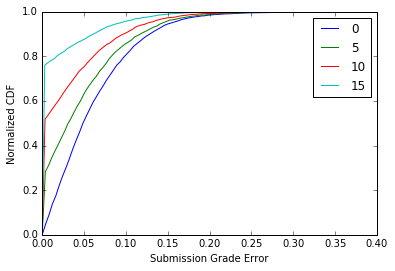
\includegraphics{vancouver-skewed.png}
		\caption{Vancouver (With Peer Quality Drawn Uniformly from the Set \{1, 5, 5, 5\})}
		\label{fig:vancouver-skewed}
	\end{figure}
	
	\begin{figure}[h]
		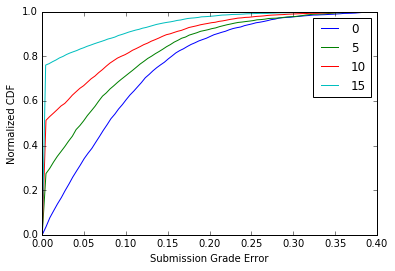
\includegraphics{vancouver-skewed-low.png}
		\caption{Vancouver (With Peer Quality Drawn Uniformly from the Set \{1, 1, 1, 5\})}
		\label{fig:vancouver-skewed-low}
	\end{figure}
	
	
	\section{Algorithms for Grading Past the Cover}
	Following the above examination, I looked into changing the algorithm for selecting submissions to provide ground truth grades for once the cover had already been graded. I tried two different types of algorithm: the first was greedy on the actual error in the grade (and thus omniscient), the second was greedy on the submission variance, as calculated by the algorithm. The latter should not have (and did not) have any impact on the results, as submission variance is not captured by our model (see Figure \ref{fig:vancouver-highest-sumbission-variance}). The first algorithm also did not noticeably improve the results (see Figure \ref{fig:vancouver-highest-grade-error}).
	
	\begin{figure}[h]
		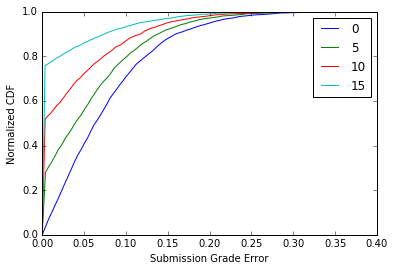
\includegraphics{vancouver-highest-grade-error}
		\caption{Vancouver with Greedy by Highest Grade Error (Omniscient)}
		\label{fig:vancouver-highest-grade-error}
	\end{figure}
	
	\begin{figure}[h]
		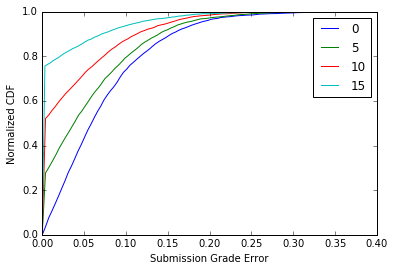
\includegraphics{vancouver-highest-submission-variance}
		\caption{Vancouver with Greedy by Highest Submission Variance (Non-Omniscient)}
		\label{fig:vancouver-highest-sumbission-variance}
	\end{figure}
	
	
	\section{Conclusion}
	Based on the results of these simulations, it does not appear that Vancouver's performance can be increased better than linearly by any of the methods for ground-truth-injection which were attempted. In fact, it appears that for these simulation parameters, Vancouver does not noticeably outperform simple averaging with ground-truth injection. It is known from results obtained by other members of the research group that Vancouver does begin to outperform simple averaging at large enough sample sizes; a possible future direction for research could be to re-run these simulations using larger sample sizes. A limited subset of these simulations was run with larger sample sizes and appeared to show no change, which is why such a direction was not pursued in this experiment. 
	
	In addition, it is worth noting that the injection of ground truth may simply outweigh any differences in the algorithms used for obtaining the non-ground-truth grades, since ground truth so powerfully affects the average error.
	
\end{document}